%%%%%%%%%%%%%%%%%%%%%%%%%%%%%%%%%%%%%%%%%%%%%%%%%%%%%%%%%%%%%%%%%%%%%%%%%%%%%%%%%%%%%%%%%%%%%%%%%%%%%%
%
%   Filename    : chapter_2.tex 
%
%   Description : This file will contain your review of related works.
%                 
%%%%%%%%%%%%%%%%%%%%%%%%%%%%%%%%%%%%%%%%%%%%%%%%%%%%%%%%%%%%%%%%%%%%%%%%%%%%%%%%%%%%%%%%%%%%%%%%%%%%%%

\chapter{Related Works}
\label{sec:relatedworks}
\begin{comment}
%
% IPR acknowledgement: the contents within this comment are from Ethel Ong's slides on RRL.
%
Guide on Writing your Related Works chapter
 
1. Identify the keywords with respect to your research
      One keyword = One document section
                Examples: 2.1 Story Generation Systems
			 2.2 Knowledge Representation

2.  Find references using these keywords

3.  For each of the references that you find,
        Check: Is it relevant to your research?
        Use their references to find more relevant works.

4. Identify a set of criteria for comparison.
       It will serve as a guide to help you focus on what to look for

5. Write a summary focusing on -
       What: A short description of the work
       How: A summary of the approach it utilized
       Findings: If applicable, provide the results
        Why: Relevance to your work

6. At the end of each section,  show a Table of Comparison of the related works 
   and your proposed project/system

\end{comment}

\section{Difficulty in Classes}
There are multiple factors which affects students' hardship in classes \cite{cmu}.
\begin{enumerate}
    \item Students may not see value in their curriculum
    \item Students does not believe their work will increase their performance
    \item Demotivated by the results and reward
    \item Restricted classroom environment
    \item Physical, mental, or other personal problems
\end{enumerate}
The examples above doesn't describe all but some of the significant factors which students are mostly affected with. There were several attempts in previous studies where some of these factors were negated with an integration of game-based learning in classrooms. \cite{watson2011} developed and introduced a video game to the classroom to teach students about World War II. Their study was able to turn static classroom environment into more friendly student-centered class and amplify the students' participation with the learning module. \cite{Hara} evaluated an effectiveness of an augmented reality application called \textit{Historic Augmented Reality Application} to increase an involvement of students by integrating a software where students can be interacted with the learning materials within the classroom environment. Their study was able to prove the improvement of students' attention span within the class with the usage of AR application and occupy them with discussions and class participation. These studies from the past have proven the game-based learning's positive effects, as well as its side effects thoroughly. It is essential to analyze and understand why game-based learning enhances the performance of some students while proving less effective for others. Understanding these factor is crucial for pinpointing what specific conditions or variables contribute to the efficacy or ineffectiveness to this approach.

\begin{comment}
    

\section{Clickers in Classroom}
There has been numerous attempt to gain back students' attention in class through the usage of an external tools. Clickers, one of the tools which was used by the teachers in the classroom settings introduced inter-activeness between the student and a teacher by promoting a classroom response systems. Clickers utilizes a remote control which a students can use to take attendance, answer a multiple choice questions, or to kick start a discussion within the class \cite{tophat:persaud}. A data in the study by \cite{clickers2010} suggests that most of the students attention alternates between an engaged and non-engaged state in a short cycle of 10-20 minutes. Within the span, the students are easily distracted by other dues such as doing homework for other class or checking their texts and social networks. The study also suggests that the usage of external tools such as Clickers to demonstrate and ask a question to the class significantly increased the attention of the students compared to the lecture-based learning materials and reduced distracted behaviors from the students. 

Unfortunately, there is always a challenge when introducing an external tools to the classroom. Firstly, the institution must have sufficient funds to approve the cost that will be associated with implementation. This involves not just a hardware but also setting up sufficient environment, such as a supplying a consistent WI-FI bandwidth across the entire classrooms. They must also invest in time in educating teachers to efficiently use certain tool in class. Additionally, an external tool - specifically Clickers has the potential to be misused by the students. A student can simply fake their friends' attendance or answer a question for them which will affect their understanding of a module, and cause a long-term effect in their studies \cite{tophat:persaud}. 

While introduction of an external tools to enhance the students' attention and create a more student-centered environment seems to be effective, it must always be approached with caution to prevent an exploitation of a tool by students. It is the responsibility of both the teacher and the creator of the tool to understand the students' frustration in class and address them accordingly. 
\end{comment}

\section{Game Based Learning}
Game based learning is a learning technique which utilizes a game either digitally or non-digitally to increase a performance of a student by enhancing critical thinking and problem solving skills and creating student-centered environment in classes \cite{tophat:tamosevicius}. Some of the known example of the game based learning includes Menti, Kahoot, Handmade Board games, and real-life games which involves physical participation of the student.

Data from several case studies involving the integration of game-based learning into classrooms shows its effectiveness in improving student performance. A study from \cite{gameOn} showed increase in students' preference and engagement from gamified lectures, and their ability to interact and share ideas reported to be more effective and amplified. Another study from \cite{watson2011} involved \textit{Making History} - a video game designed with an educational purpose to teach students the history of World War II. This case study showed how the integration of game-based learning into a standard American classroom was able to convert the restricted teacher-centered classroom where students were mostly passive into a more student-centered environment which made students more engaged and less hesitant to share their ideas to the class.  

While game-based learning does provide positive effects toward students, there are side effects which may occur if not integrated properly to the class. In recent years, there has been an increase in phenomena of \textit{Gaming the System}, where learners attempt to exploit the education system to achieve a high performance rather than attempting to absorb the lessons \cite{baker2008}. It is important to understand why students choose to game the system to create a educational that students do not attempt to exploit it.

According to \cite{malone1980fun} in his study on what makes things fun to learn, there are certain criteria which needs to be considered to create an effective game for education. 1. The game must have clear goal and must be compelling, 2. The player must know if they are getting closer to the goal, 3. Game should provide varying difficulty for the varying skill levels of the players. Another insight from \cite{mozelius2017} in the perspective of the games that will be used for education must be 1. Not to costly, and must be easy to install, 2. The game should be playable under 40 minutes to be used in a classroom settings, 3. If not, the game is better to be used as a homework instead. These criteria from the previous studies must be carefully observed and integrated into the project accordingly to avoid exploits from the students.  

\section{Affective Learning and World War II History}
According to Mahadeo and Nepal (2023), a teaching method that recognizes the vitality of emotions in learning improves students' experience, creating a positive and effective outcome. Affective Learning, as defined, is the process of learning skills and attitudes through emotional engagement. It enhances curiosity and enthusiasm in learning outcomes that foster a deeper understanding of the context with meaningful retention of information. It is an approach that tailors to cognitive and emotional dependency to promote holistic and impactful learning experiences. Nurturing positive emotional experiences can improve student engagement, critical thinking, and academic performance by creating a transformative learning experience that allows personal and educational growth.

The strategy of using Affective Learning in teaching World War II History can affect how the students can see the gravity of the effects of war on the country and the people without having to experience it and by only seeing it through the lens of those who lived it. A study by Kim et al. (2019) showed the hardships of comfort women during World War II. The Japanese Military during World War II created comfort stations that used women as tools for relief, stripping the dignity and freedom of the comfort women. The study used male and female students of diverse ethnicities to interview comfort women survivors who narrated their experiences. One of the students said that he learned the facts about comfort women in class, but hearing the reality from the person who survived made the history "more real." According to Waters and Russell III (2012), the violation of human rights in the context of history should be taught in social studies classrooms to help students become better citizens. Discussing and exploring the issues of human rights violations in the context of World War II history helps students conceptualize and identify current human rights violations while stating that mere recognition of injustices is not enough to pursue actions.

\section{Historic Augmented Reality Application (HARA)}
There has been several studies on applying augmented reality (AR) technology into education to amplify the learning of the students and create an immersive environment for them \cite{ARVRRome}. Although there are numerous studies from various parts of the world, there are few papers discussing the application of AR technology in school settings in the Philippines. 

Historic Augmented Reality Application (HARA) is an application developed in the Philippines which aims to teach students the Philippines-American colonization period through immersive story telling \cite{Hara}. The application aimed to teach students the three distinct event during the American colonization, namely the battle of manila bay, mock battle of manila, and the first shot in Philippines-American war. 

HARA is a mobile-based application integrated with AR technology, and the decision was made to develop it using the Unity and Vuforia engine. This choice was influenced by Unity's capability to publish across over 25 platforms compared to other suitable mobile development platforms such as Android Studio, and technical aspect of how Vuforia engine is easily co operable with Unity engine was another factor in the decision making. The HARA relies on image recognition of the predefined set images through the cameras of the mobile phones, after which the application overlays a 3D animated scene displaying the event shown in the images. The development of the HARA lasted from May to October of year 2018, with first four months spent on development and beta release of the application, and final two for user evaluation and modification. 

HARA was the first application in the Philippines which utilizes augmented reality with 3D animated scenes to be used to teach history in a classroom setting. As a pioneering application in the field, to ensure the standard in the field of human-computer interaction field, the application usability was surveyed with a questionnaire based from the works of Guimarães and Martins which is used to evaluate AR application in terms of variables such as effectiveness, efficiency, and such by the co-designers of the application. The application received 82 percentage markings on its effectiveness, but received poor markings on satisfaction - 51, and efficiency - 43 from the co-designers due to factors such as slow animation and loading time. While the designers weren't fully satisfied with the application, the overall qualitative feedback from the users were positive. The application received a high overall markings of 4.2 out of 5, and got positive reviews from both students and teachers. Overall, the HARA shows how the AR technology is a promising tool in a field of education to effectively create immersive environment for the students.

\section{EON-XR: The Urban Planning of Rome}
With the growth of popularity of video games worldwide and the advancement in the field of Augmented and Virtual reality \cite{enterpriseappstoday2023}, Augmented Reality (AR) is no longer a technology that is foreign towards the young audiences such as high school and college students around the world. With student's apparent lack of motivation to study \cite{medium:mosley} and their hardship in classes, there has been numerous case studies on integrating gamification into education to boost the student's performance in class \cite{watson2011}. 

The study on \textit{EON-XR}, stands out among similar works as it is a simulation video game embedded with both Augmented and Virtual reality technology and was developed to be used for educational purposes \cite{ARVRRome}. The application was developed for mobile settings using Unity with Vuforia engine plug-ins for AR. The models of the buildings and characters were made with a 3DS Max modeling tool, maximizing the details of each assets for greater user immersion. 

The students were allowed to utilize the AR portion of the application to observe the visualization of the city elements with an optional description on the side to further enhance the explanation. This activity was told to increase the educational value of the game, and is to amplify the immersion of the era for the students. Aside from its AR feature, the EON-XR application also provides the user with a virtual reality (VR) simulation to allow them to walk around the cities of ancient Rome and visit notable landmarks such as The Colosseum on foot. The user can roam around a pre-designed city or build a city on their own to create an immersive simulation to their liking. To increase the historical potential of the game, the developers added a scroll with information of notable buildings inside them which the users can read in first person upon entering the buildings. \textit{EON-XR} shows a strong evidence of AR and VR being utilized to create immersive environment for the users, and create suitable environment around them to absorb the information efficiently.


\section{A Deep Dive into Immersive Technology}
Immersive technology, which includes AR and VR, have an increased in scholarly attention through the years. With that attention, only a few studies have been done to discuss the current state of this kind of research. A literature review was done from 54 rigorously selected articles and their findings were summarized into one study; all to show the current state of immersive technology, and to give light on gaps on research \cite{suh2018}.

The study summarized and combined results and data from the set of studied ariticles into multiple tables and figures that show aspects of both VR and AR \cite{suh2018}. The literature review summarized that immersive technology is good at increasing learning effectiveness and engagement while also improving attitudes at said learning materials; the study also discussed that, to increase immersion and effectiveness, it is better to have interactive elements, even better they are collaborative in nature \cite{suh2018}.

The literature review delved deep into both AR and VR technology and points out key concepts that are important in the application of those technology. The study's findings will definately help in guiding the researchers in the creation of the simulation and to create an even more immersive and effective AR experience. Lastly, the study created a framework from which our project can be built upon as seen from the figure below \cite{suh2018}.

\begin{figure}[h]
    \centering
    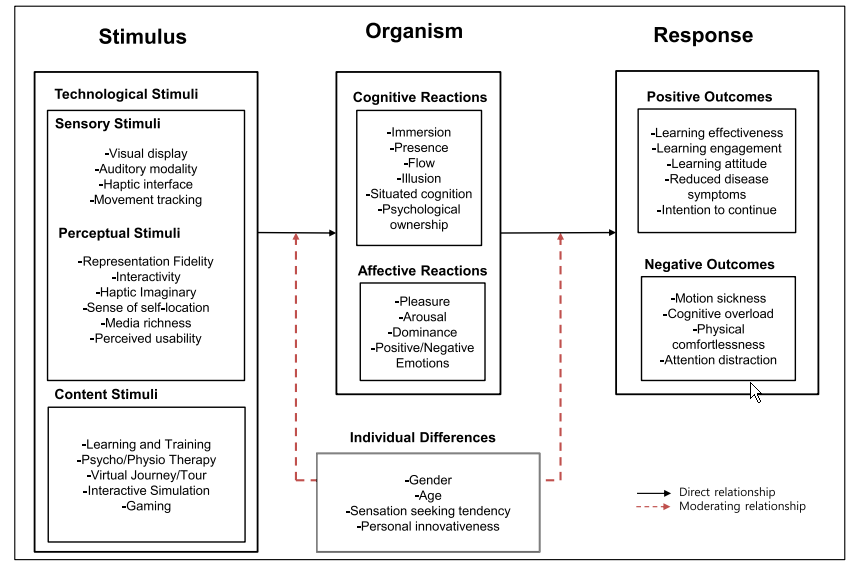
\includegraphics[width=0.8\textwidth]{figures/ImmersiveFramework.png}
    \caption{Immersive Technology Framework}
\end{figure}

\section{User-centric View on Immersion in Augmented Reality Games}

The term \textit{immersion} can have different definitions depending on the context in which it is used. In Virtual Reality (VR), immersion refers to a user's perception and sense of presence in a computer-generated world \cite{immersionAR}. This is achieved through surrounding the  
However, what does immersion signify in the context of Augmented Reality (AR) technology? 













